\section{Rotationsschwingung}
Die Rotationsschwingung ist wie das horizontale und vertikale Federpendel
ein einfach harmonisches Schwingungssystem. Dies zeigt sich direkt an deren
Differentialgleichung. Da es sich hier um eine Rotationsbewegung handelt 
wird diese mittels der Momente gebildet
\[ \boxed{\vec{M}_{\Sigma} 
	= \vec{M}_R + \vec{M}_F 
	= I_s \cdot \ddot{\theta} + \kappa \cdot \theta = 0
} \]
\[ \boxed{\theta(t) = \theta_{max} \cdot \cos(\omega \cdot t + \phi)} \]

\begin{figure}[h!]
	\centering
	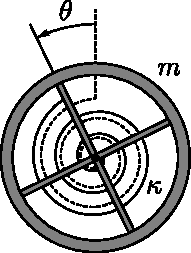
\includegraphics[scale=0.75]{../fig/rotationspendel.pdf}
	\caption{Rotationspendel}
\end{figure}

\paragraph{Spiralfeder} Im Unterschied zur Linearfeder wird die Spiralfeder
nicht mittels eines $k=\left[\frac{N}{m}\right]$ sondern mittels eines
$\kappa=\left[Nm\right]$ beschrieben.

\paragraph{Für kleine Winkel} Ist die Auslenkung $\theta$ klein, dann gelten
 die folgenden Formeln.
\[ \boxed{\kappa = \sum_{1}^{n} \left(k_n \cdot {r_n}^2\right)} \]
\[ \boxed{\kappa = k_1 \cdot {r_1}^2 + k_2 \cdot {r_2}^2 + \dots } \qquad 
\text{$r$: Abstand Feder zu Drehpunkt} \]
\[ \boxed{\omega = \sqrt{\frac{\kappa}{I}}} \]
\[ \boxed{f = \frac{\sqrt{\dfrac{\kappa}{I}}}{2 \pi}} \]
\[ \boxed{T = 2 \cdot \pi \cdot \sqrt{\frac{I}{\kappa}}} \]
